% Presentación de PULSO. Compilar desde docs/latex/presentacion:
%   latexmk -lualatex presentacion.tex
\documentclass[aspectratio=169,11pt]{beamer}
\usetheme[progressbar=frametitle,numbering=fraction,block=fill]{metropolis}
\usepackage{fontspec}
\usepackage[spanish,es-noshorthands,es-nodecimaldot]{babel}
\usepackage{booktabs}
\usepackage{tikz}
\usetikzlibrary{arrows.meta,positioning}
\setmonofont{DejaVu Sans Mono}[Scale=0.8]
\graphicspath{{../figuras/}{../../../figures/}}

\definecolor{azul}{HTML}{2563A8}
\definecolor{rojo}{HTML}{C2362B}
\definecolor{verde}{HTML}{2F7D5B}
\definecolor{gris}{HTML}{5F6B77}
\setbeamercolor{frametitle}{bg=azul}
\setbeamercolor{progress bar}{fg=rojo}
\setbeamercolor{alerted text}{fg=rojo}
\setbeamercolor{block title}{bg=azul!15,fg=black}
\setbeamercolor{block body}{bg=azul!5}

\title{PULSO}
\subtitle{Pagos, Umbrales, Liquidez y Sincronización Operativa\\[2pt]
\footnotesize Redes complejas, sincronización y riesgo en sistemas de pagos digitales}
\author{Juan Diego Martínez Ayala \\ \small Dirección: Jhon Hernán Díaz Forero}
\institute{\small Semillero de Modelamiento de Sistemas Complejos y Física Computacional}
\date{Noviembre de 2026 · software v3.0.0}

\tikzset{
  c/.style={draw=#1,fill=#1!7,rounded corners=3pt,align=center,
    minimum width=11.5cm,minimum height=0.9cm,font=\small},
  etapa/.style={draw=#1,fill=#1!6,rounded corners=3pt,align=center,
    minimum width=2.7cm,minimum height=1.1cm,font=\small},
  f/.style={-{Stealth[length=2.5mm]},thick,gris}}

\begin{document}
\maketitle

\begin{frame}{Contenido}
\begin{enumerate}
\item \textbf{Planteamiento}: problema, fundamento físico y aporte
\item \textbf{Modelo y desarrollo}: las seis tareas de la propuesta
\item \textbf{Resultados}: validación, riesgo sistémico y riesgo crediticio
\item \textbf{Implementación}: arquitectura, aplicación y ejecución
\end{enumerate}
\end{frame}

% ===================================================================
\section{Planteamiento}

\begin{frame}{Interdependencia en los sistemas de pagos}
\begin{columns}[T]
\column{0.55\textwidth}
\begin{itemize}
\item Salarios, arriendos, facturas y cuotas se liquidan en \textbf{sistemas de pagos
digitales}; en Colombia, por ejemplo, \textbf{Bre-B}.
\item La capacidad de pago de cada agente depende de los ingresos que recibe: los
pagos conforman una \alert{red}.
\item \textbf{Liquidez}: disponibilidad inmediata de recursos. Su insuficiencia es un
\textbf{déficit}; un déficit excesivo conduce al \textbf{impago}.
\item Un impago reduce el ingreso de otros agentes y puede propagarse:
\alert{riesgo sistémico}.
\end{itemize}
\column{0.42\textwidth}
\centering
\begin{tikzpicture}[n/.style={circle,draw=azul,fill=azul!10,minimum size=7mm},
  e/.style={-{Stealth[length=2mm]},thick}]
\node[n,fill=rojo!40] (a) at (0,0) {A};
\node[n] (b) at (1.8,0.8) {B};
\node[n] (c) at (1.8,-0.8) {C};
\node[n] (d) at (3.6,0) {D};
\draw[e] (a)--(b); \draw[e] (a)--(c); \draw[e] (b)--(d); \draw[e] (c)--(d);
\node[font=\scriptsize,align=center] at (1.8,-1.7) {El impago de A reduce el ingreso de B y C\\y compromete la liquidez de D};
\end{tikzpicture}
\end{columns}
\end{frame}

\begin{frame}{Ciclos de pago y desfase}
\begin{columns}[c]
\column{0.42\textwidth}
\begin{itemize}
\item Los pagos ocurren en \textbf{ciclos}: nómina quincenal o mensual, plazos de
facturación, fechas de cuota.
\item Un desfase entre la fecha de ingreso y la de las obligaciones exige un mayor
colchón de liquidez.
\item Un ingreso \alert{desfasado} genera estrés financiero aunque su monto no cambie.
\end{itemize}
\column{0.56\textwidth}
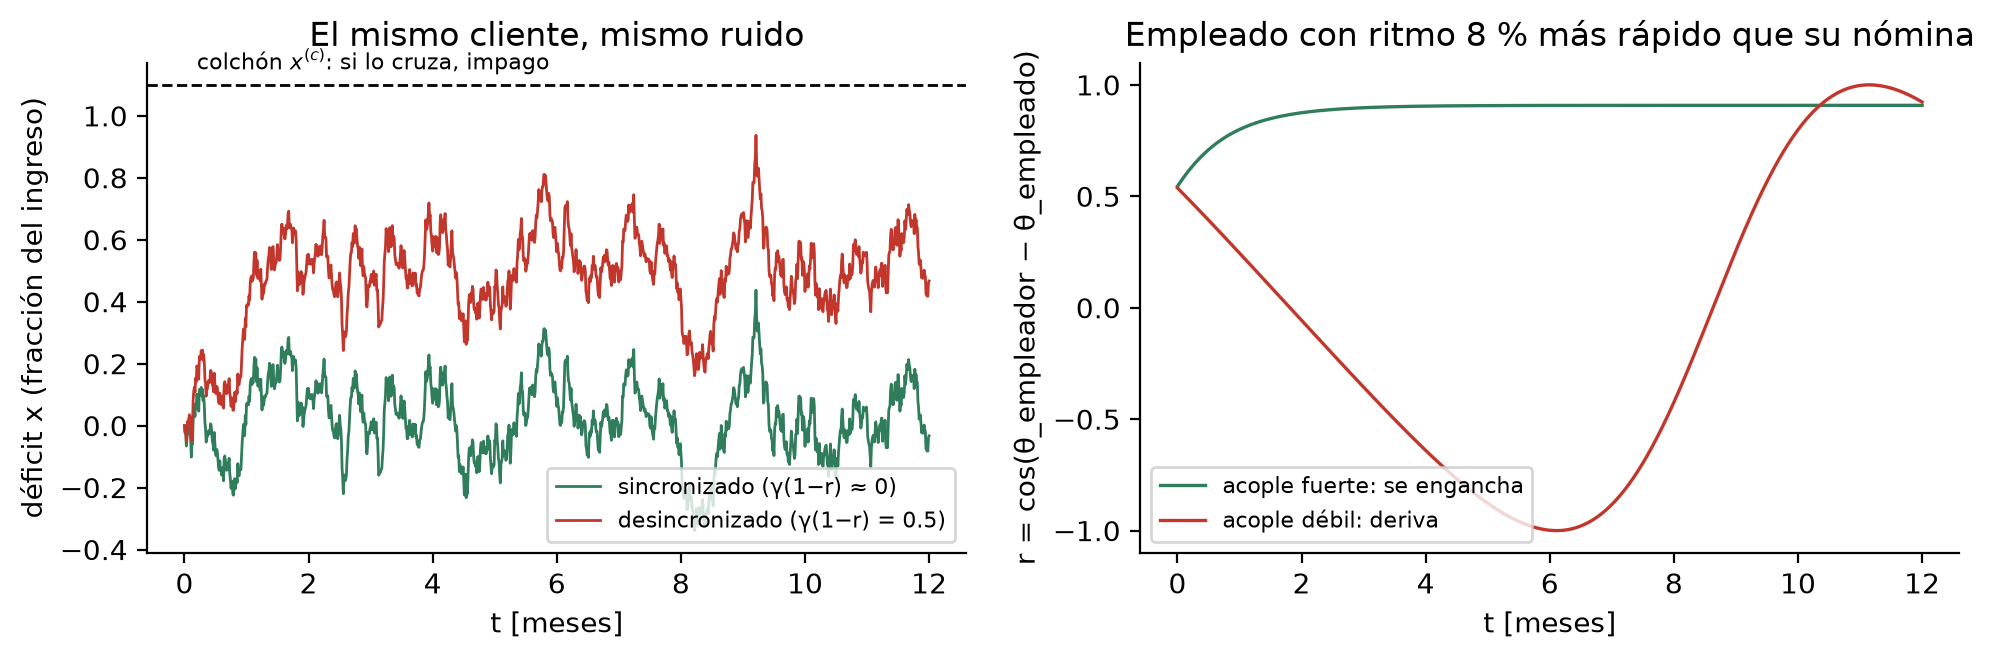
\includegraphics[width=\textwidth]{concepto_deficit_y_ritmo.png}
\end{columns}
\end{frame}

\begin{frame}{Pregunta de investigación}
\begin{block}{Riesgo sistémico (tareas 1–5)}
Modelo físico-matemático de una red de pagos en el que el déficit se propaga, los
ciclos de pago se sincronizan y las entidades incurren en impago al superar un umbral;
modelos de aprendizaje automático que anticipan el colapso.
\end{block}
\begin{alertblock}{Riesgo crediticio (tarea 6)}
¿La \textbf{dinámica} de la red de pagos de los clientes de un banco, medida como la
sincronización de sus ciclos de pago, aporta información sobre el impago adicional a
la del \textbf{score clásico} y a la de la \textbf{estructura estática} de la red?
\end{alertblock}
\end{frame}

\begin{frame}{Fundamento físico}
\begin{columns}[T]
\column{0.5\textwidth}
\textbf{Componentes del modelo}
\begin{enumerate}
\item \textbf{Red}: $W_{ij}$, pago de $j$ hacia $i$ por ciclo.
\item \textbf{Variables de estado}: déficit $x_i$ y fase del ciclo de pagos $\theta_i$.
\item \textbf{Dinámica}: contagio del déficit, sincronización de Kuramoto y umbral de
impago.
\end{enumerate}
\column{0.48\textwidth}
\footnotesize
\begin{tabular}{ll}
\toprule
Concepto físico & Concepto financiero \\
\midrule
Nodo & Entidad o cliente \\
Arista $W_{ij}$ & Pago de $j$ a $i$ \\
Relajación & Corrección del déficit \\
Acoplamiento & Contagio \\
Fase $\theta$ & Momento del ciclo \\
Parámetro de orden $r$ & Sincronización de pagos \\
Umbral & Colchón de liquidez \\
Avalancha & Cascada de impagos \\
\bottomrule
\end{tabular}
\end{columns}
\end{frame}

\begin{frame}{Aplicaciones y aporte}
\small
\begin{columns}[T]
\column{0.5\textwidth}
\textbf{Aplicaciones}
\begin{itemize}
\item \textbf{Supervisión}: identificación de entidades sistémicas, simulación de
choques e indicadores de alerta temprana basados en la sincronización global.
\item \textbf{Gestión de cartera}: riesgo no capturado por el score y escenarios de
quiebra de empleadores.
\item \textbf{Investigación}: hipótesis falsable entre física estadística y finanzas.
\end{itemize}
\column{0.48\textwidth}
\textbf{Aporte respecto a la literatura}
\begin{itemize}
\item El uso de redes en riesgo crediticio está documentado, casi siempre con
variables \textbf{estáticas} (Letizia y Lillo, 2019; Tobback et al., 2017).
\item Aporte: variables \textbf{dinámicas} de sincronización estimadas desde
transacciones, evaluadas frente a un \textbf{control nulo}.
\item Parámetros \alert{ilustrativos}: se valida el mecanismo, no su magnitud real.
\end{itemize}
\end{columns}
\end{frame}

% ===================================================================
\section{Modelo y desarrollo}

\begin{frame}{Estructura del proyecto}
\centering
\begin{tikzpicture}[node distance=0.55cm]
\node[etapa=azul] (a) {1. Red y\\déficit};
\node[etapa=azul,right=of a] (b) {2. Difusión y\\estabilidad};
\node[etapa=azul,right=of b] (c) {3. Sincronización\\(Kuramoto)};
\node[etapa=azul,below=0.8cm of c] (d) {4. Impagos y\\cascadas};
\node[etapa=azul,left=of d] (e) {5. Experimentos y\\predicción};
\node[etapa=rojo,left=of e] (g) {6. Riesgo\\crediticio};
\draw[f] (a)--(b); \draw[f] (b)--(c); \draw[f] (c)--(d); \draw[f] (d)--(e); \draw[f] (e)--(g);
\end{tikzpicture}

\vspace{0.4cm}
\small Criterio de diseño: al anular los términos nuevos, el modelo coincide
\textbf{exactamente} con el de la tarea anterior; las pruebas automáticas lo verifican.
\end{frame}

\begin{frame}{Formulación del modelo (tareas 1–4)}
\footnotesize
\[
\frac{dx_i}{dt} = \underbrace{-\alpha x_i}_{\text{corrección}}
+ \underbrace{\beta\sum_j W_{ij}x_j}_{\text{contagio}}
\underbrace{- D_0(Lx)_i}_{\text{redistribución}}
+ \underbrace{\gamma\,k_i(1-r_i)}_{\text{ingreso desfasado}} + \eta_i(t)
\]
\[
\frac{d\theta_i}{dt} = \omega_i + \frac{K}{\langle k\rangle}\sum_j W_{ij}\sin(\theta_j-\theta_i),
\qquad x_i > x_i^{(c)} \Rightarrow \text{impago}
\]
\begin{itemize}
\item \textbf{Tarea 1}: índice de amplificación $R=\beta\rho(W)/\alpha$; la red es
estable si $R<1$ (Perron–Frobenius).
\item \textbf{Tarea 2}: Laplaciano $L=D_\text{out}-W$ conservativo; estabilidad
$\sigma=\max\mathrm{Re}\,\lambda$, recuperación $\tau_\text{rec}=-1/\sigma$, $\lambda_2$.
\item \textbf{Tarea 3}: parámetro de orden $r=|\langle e^{i\theta}\rangle|$ y coherencia
local $r_i$.
\item \textbf{Tarea 4}: colchones, choques y cascada; comparación con Eisenberg–Noe,
DebtRank y Watts.
\end{itemize}
\end{frame}

\begin{frame}{Tareas 1 y 2: estabilidad de la red}
\begin{columns}[c]
\column{0.6\textwidth}
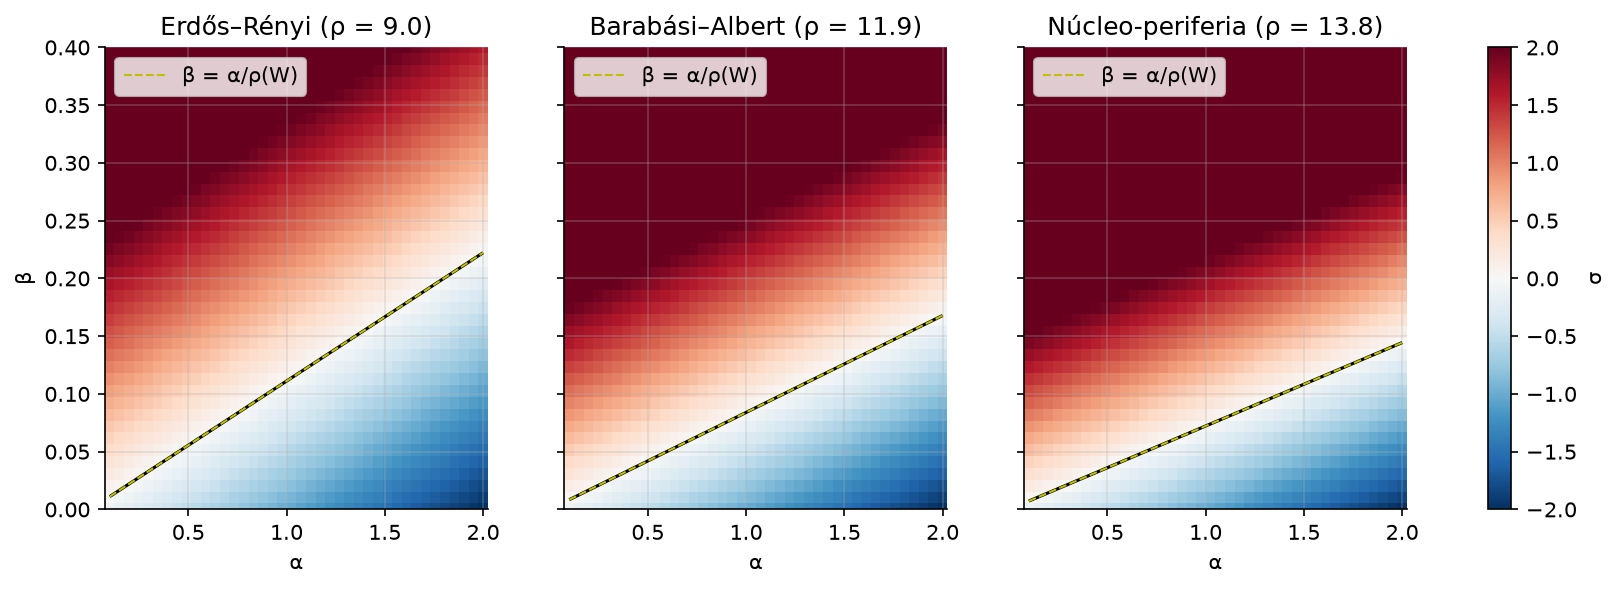
\includegraphics[width=\textwidth]{fase1_diagrama_alpha_beta.png}
\column{0.38\textwidth}
\footnotesize
\begin{itemize}
\item La línea punteada corresponde a $R=1$.
\item Las redes más concentradas (mayor $\rho$) pierden estabilidad antes.
\item La redistribución $D_0$ amplía la región estable más allá de $R=1$.
\end{itemize}
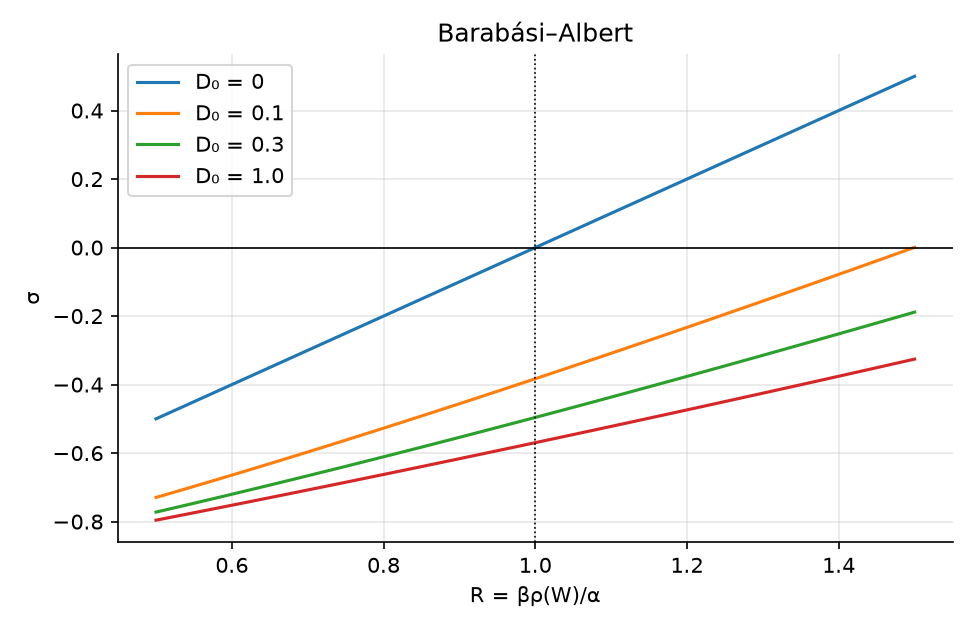
\includegraphics[width=0.85\textwidth]{fase2_D0_umbral.png}
\end{columns}
\end{frame}

\begin{frame}{Tareas 3 y 4: sincronización y cascadas de impago}
\begin{columns}[c]
\column{0.49\textwidth}
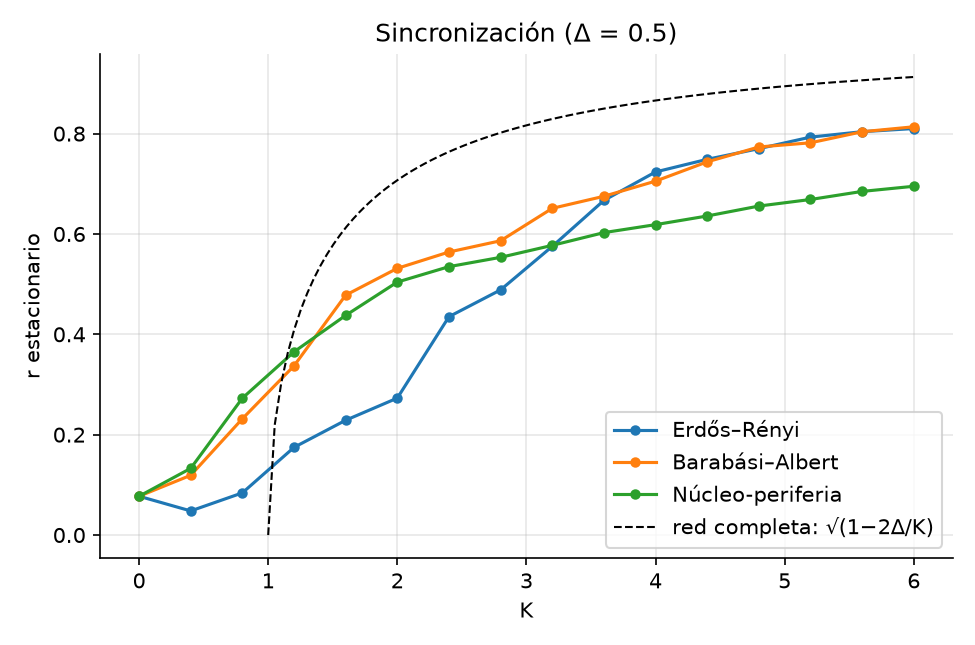
\includegraphics[width=\textwidth]{fase3_r_vs_K.png}
\small Red completa: $r=\sqrt{1-2\Delta/K}$ (simulado 0.7076; teórico 0.7071).
\column{0.49\textwidth}
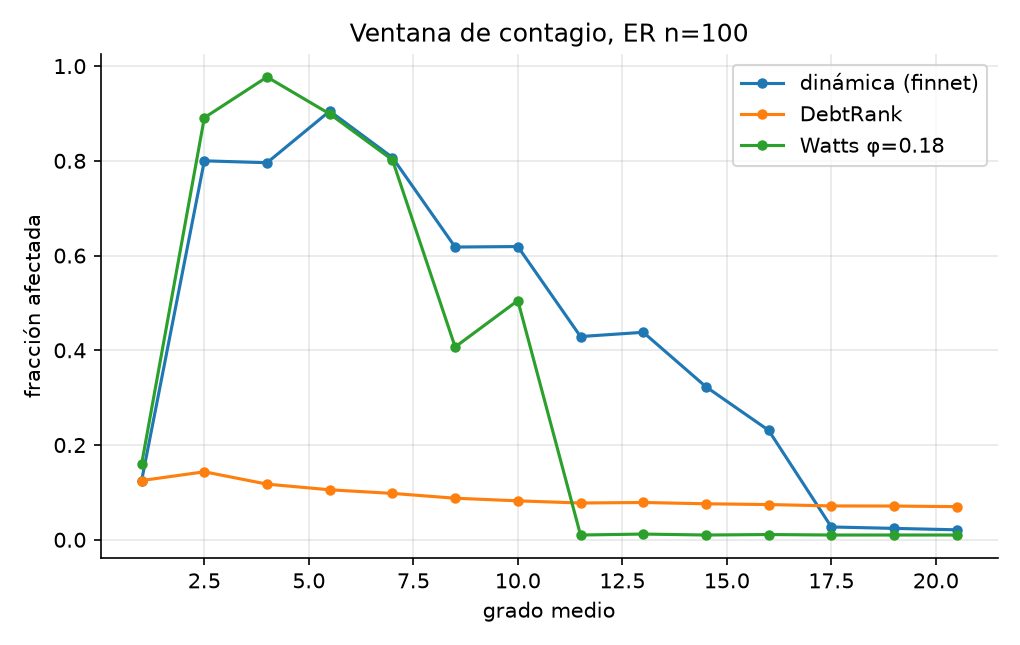
\includegraphics[width=\textwidth]{fase4_ventana_contagio.png}
\small Ventana de contagio: las cascadas son máximas con conectividad intermedia.
\end{columns}
\end{frame}

\begin{frame}{Tarea 5: predicción a partir de 20\,000 escenarios}
\begin{columns}[T]
\column{0.45\textwidth}
\begin{itemize}
\item 300 redes y 20\,000 escenarios (hipercubo latino con mayor densidad cerca de
$R=1$).
\item Conjunto de datos reproducible bit a bit (Parquet).
\item Validación \textbf{GroupKFold por red}.
\item Predicción unas $10^4$ veces más rápida que la simulación.
\end{itemize}
\column{0.53\textwidth}
\footnotesize
\begin{tabular}{lll}
\toprule
Modelo & Objetivo & Métrica \\
\midrule
Logística & colapso & AUC 0.957 \\
XGBoost & colapso & AUC \textbf{0.980} \\
XGBoost & cascada por entidad & $R^2$ 0.50 \\
GCN & cascada por entidad & $R^2$ \textbf{0.60} \\
PINN & parámetros & $\gamma,K$: error $<1\%$ \\
\bottomrule
\end{tabular}
\end{columns}
\end{frame}

\begin{frame}{Tarea 6: cartera multicapa de un banco}
\begin{columns}[c]
\column{0.5\textwidth}
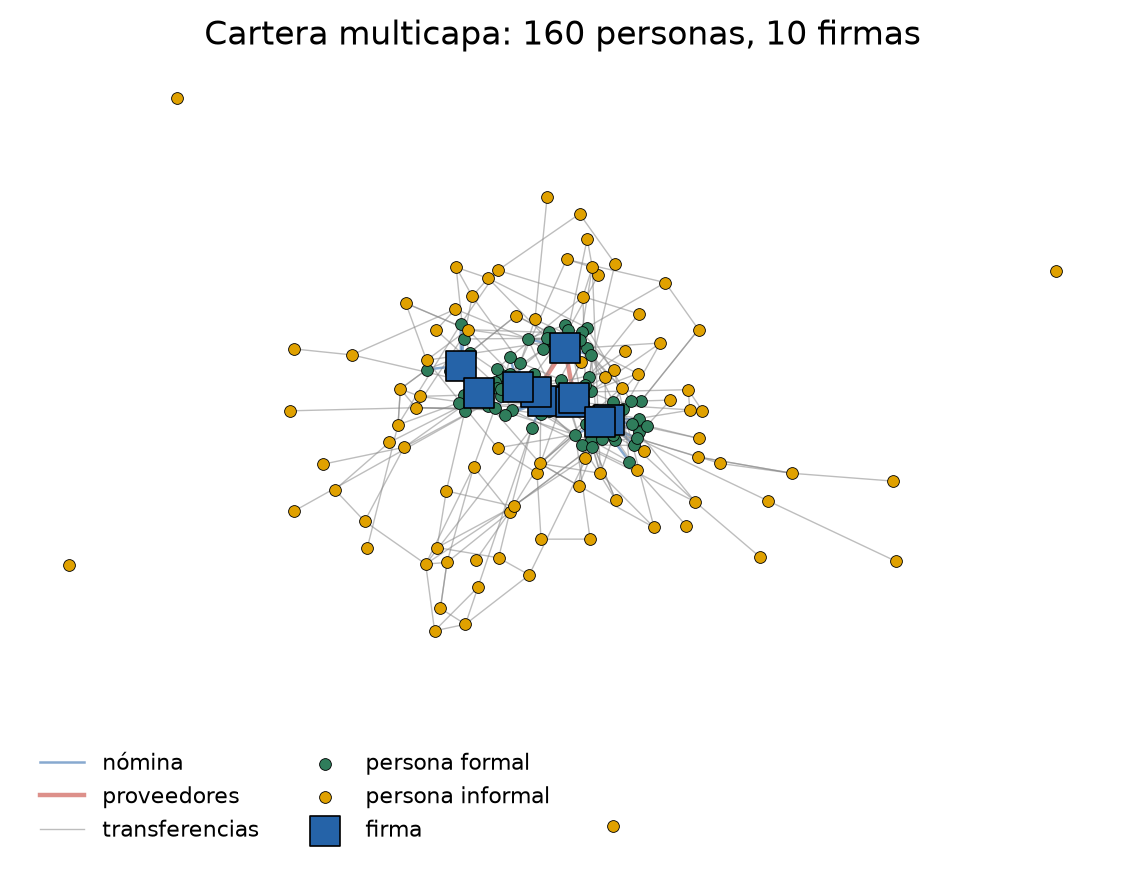
\includegraphics[width=\textwidth]{tarea6_red_multicapa.png}
\column{0.48\textwidth}
\small
\begin{itemize}
\item 2000 personas (55~\% informales) y 100 firmas.
\item Tres capas: \textcolor{azul}{\textbf{nómina}}, \textcolor{rojo}{\textbf{proveedores}}
y \textbf{transferencias}.
\item Variables clásicas y una \textbf{PD verdadera} no observable
(\texttt{truth\_*}), excluida de los modelos por validación de esquema.
\item Tiempo en meses; déficit expresado como fracción del ingreso.
\end{itemize}
\end{columns}
\end{frame}

\begin{frame}{Modelo dinámico multicapa}
\[
\dot x_i = -\alpha x_i + \sum_\ell\beta_\ell\sum_j\frac{W^\ell_{ij}}{s_i}x_j
+ \gamma\frac{k_i}{s_i}(1-r_i) + \sigma\xi_i,
\qquad
\dot\theta_i = \omega_i + \sum_\ell K_\ell\sum_j\frac{W^\ell_{ij}}{k_i}\sin(\theta_j-\theta_i)
\]
\begin{itemize}
\item Contagio y acoplamiento \textbf{por capa}; matrices dispersas (una cartera se
simula en menos de 1~s).
\item Colchón $\propto \mathrm{PD}_i^{-\kappa}$; impagos idiosincráticos con tasa
$-\ln(1-\mathrm{PD})/12$ por mes.
\item Choque adicional: \textbf{quiebra} de un empleador.
\item Con una sola capa, el modelo coincide \textbf{exactamente} con la versión 1.
\end{itemize}
\end{frame}

\begin{frame}{Estimación a partir de transacciones}
\begin{columns}[c]
\column{0.58\textwidth}
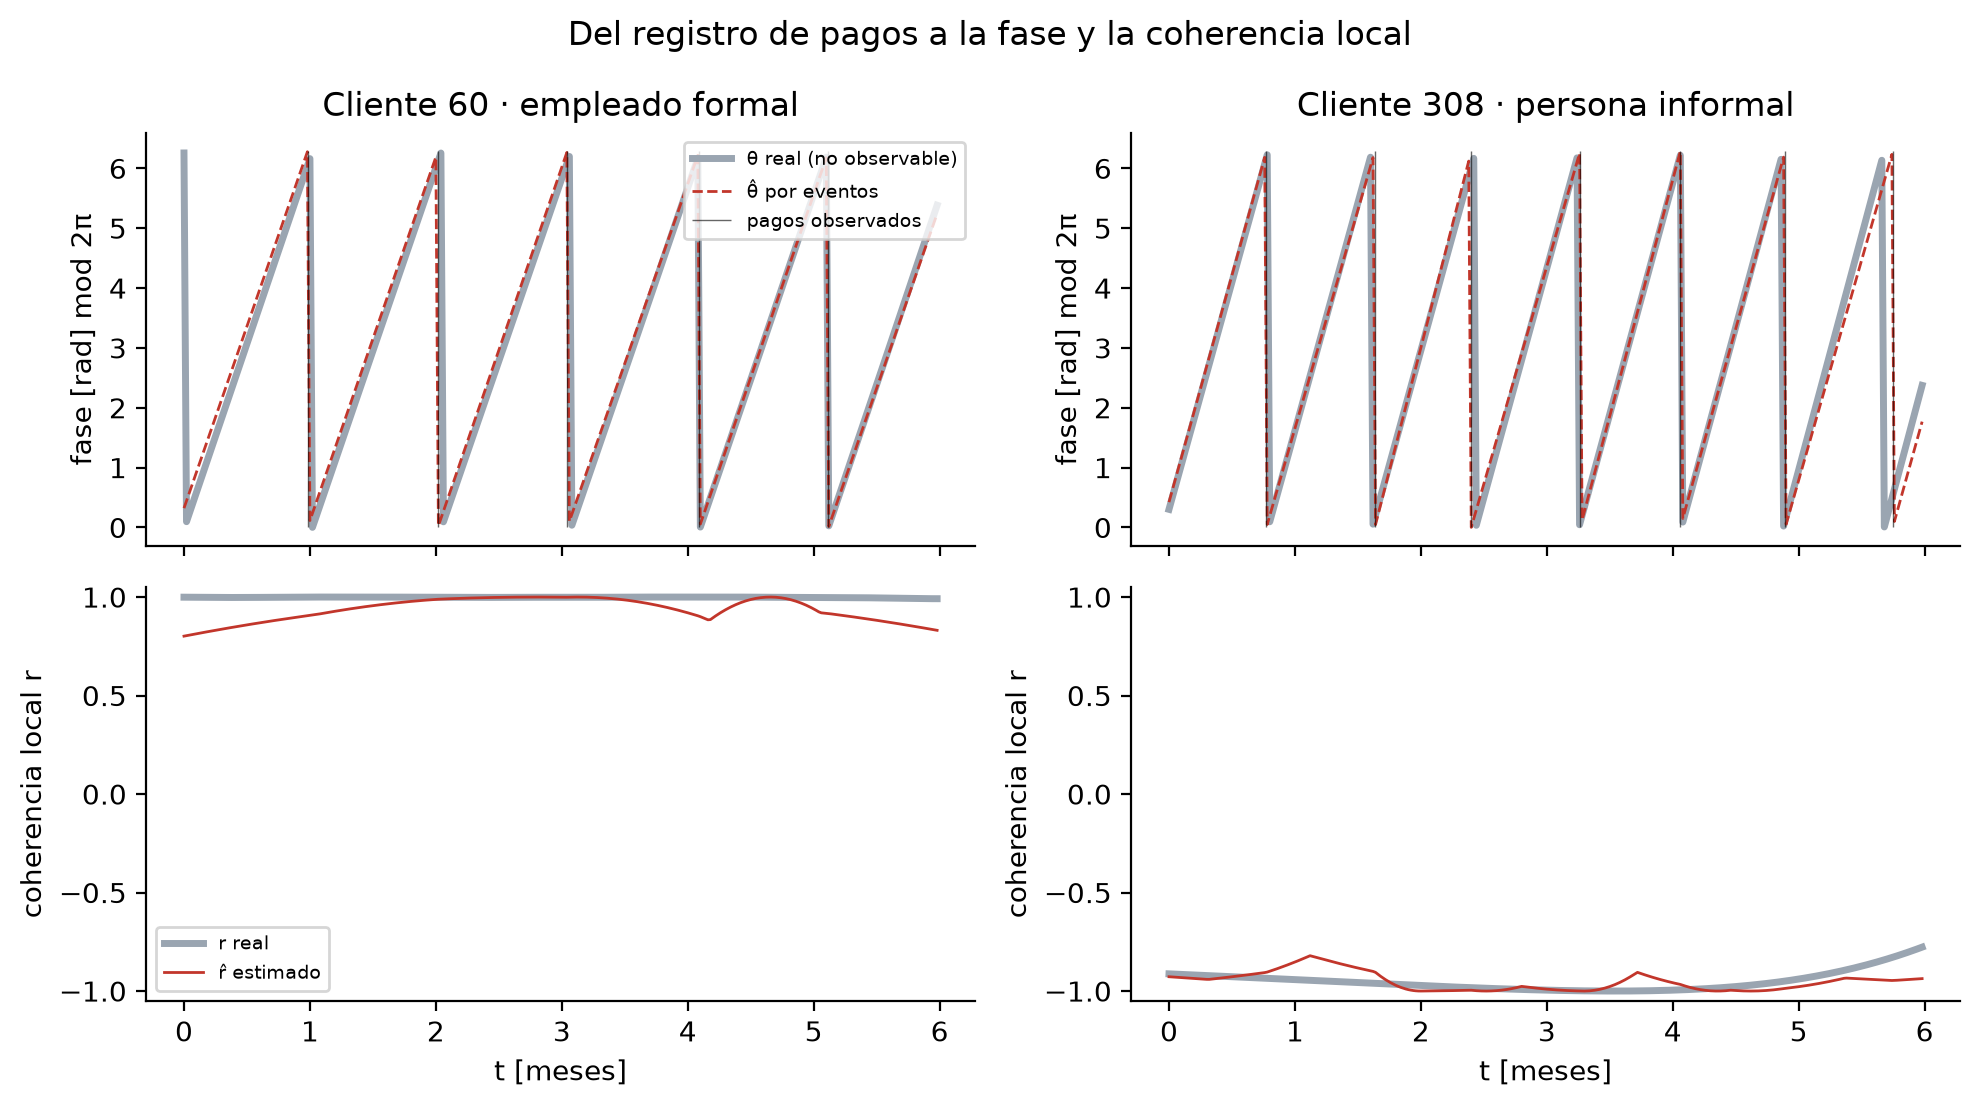
\includegraphics[width=\textwidth]{tarea6_fase_eventos.png}
\column{0.4\textwidth}
\small
\begin{itemize}
\item Cada cruce de fase genera un ciclo de pagos con fecha.
\item \textbf{Fase por eventos} (Pikovsky et al., 2001):
\[\hat\theta = 2\pi\Big(k+\tfrac{t-t_k}{t_{k+1}-t_k}\Big)\]
\item Correlación entre $\hat r_i$ estimada y $r_i$ del modelo: $>0.8$.
\item La estimación no utiliza la verdad del terreno.
\end{itemize}
\end{columns}
\end{frame}

\begin{frame}{Diseño experimental}
\begin{columns}[T]
\column{0.5\textwidth}
\textbf{Conjuntos de variables}
\begin{enumerate}
\item \textbf{Clásico}: ingreso, endeudamiento, moras, antigüedad, formalidad.
\item \textbf{Red estática}: composición y concentración del ingreso, PageRank,
condición del empleador y de los pagadores.
\item \textbf{Red dinámica}: $\hat r$ y su variabilidad, desfase, desajuste de
frecuencia, irregularidad de ciclos, pagadores que cesaron sus pagos.
\end{enumerate}
\column{0.48\textwidth}
\begin{block}{Protocolo}
\small
\begin{itemize}
\item Observación de 6 meses; impago en los 12 meses siguientes.
\item 20 carteras por régimen; GroupKFold por cartera.
\item \alert{Régimen nulo}: mismos clientes y sorteos aleatorios, sin efecto de la red
sobre el déficit.
\item Diferencias \textbf{pareadas} por partición con IC del 95~\%.
\end{itemize}
\end{block}
\end{columns}
\end{frame}

% ===================================================================
\section{Resultados}

\begin{frame}{Validación numérica}
\footnotesize
\begin{tabular}{ll}
\toprule
Verificación & Resultado \\
\midrule
RK4 frente a $e^{Mt}x_0$ & error $<10^{-6}$ \\
Conservación bajo difusión & $<10^{-10}$ \\
Tasa de recuperación $\alpha+D_0\lambda_2$ & 1~\% \\
Kuramoto en red completa & 0.7076 frente a 0.7071 \\
Modelo multicapa (una capa) frente a versión 1 & idénticos \\
Varianza de Ornstein–Uhlenbeck & 10~\% \\
$\hat W$ y frecuencias estimadas desde transacciones & error mediano $<5$~\% \\
$\hat r_i$ frente a $r_i$ & correlación $>0.8$ \\
\bottomrule
\end{tabular}

\vspace{0.3cm}
\textbf{127 pruebas automáticas superadas.}
\end{frame}

\begin{frame}{Resultado principal}
\centering
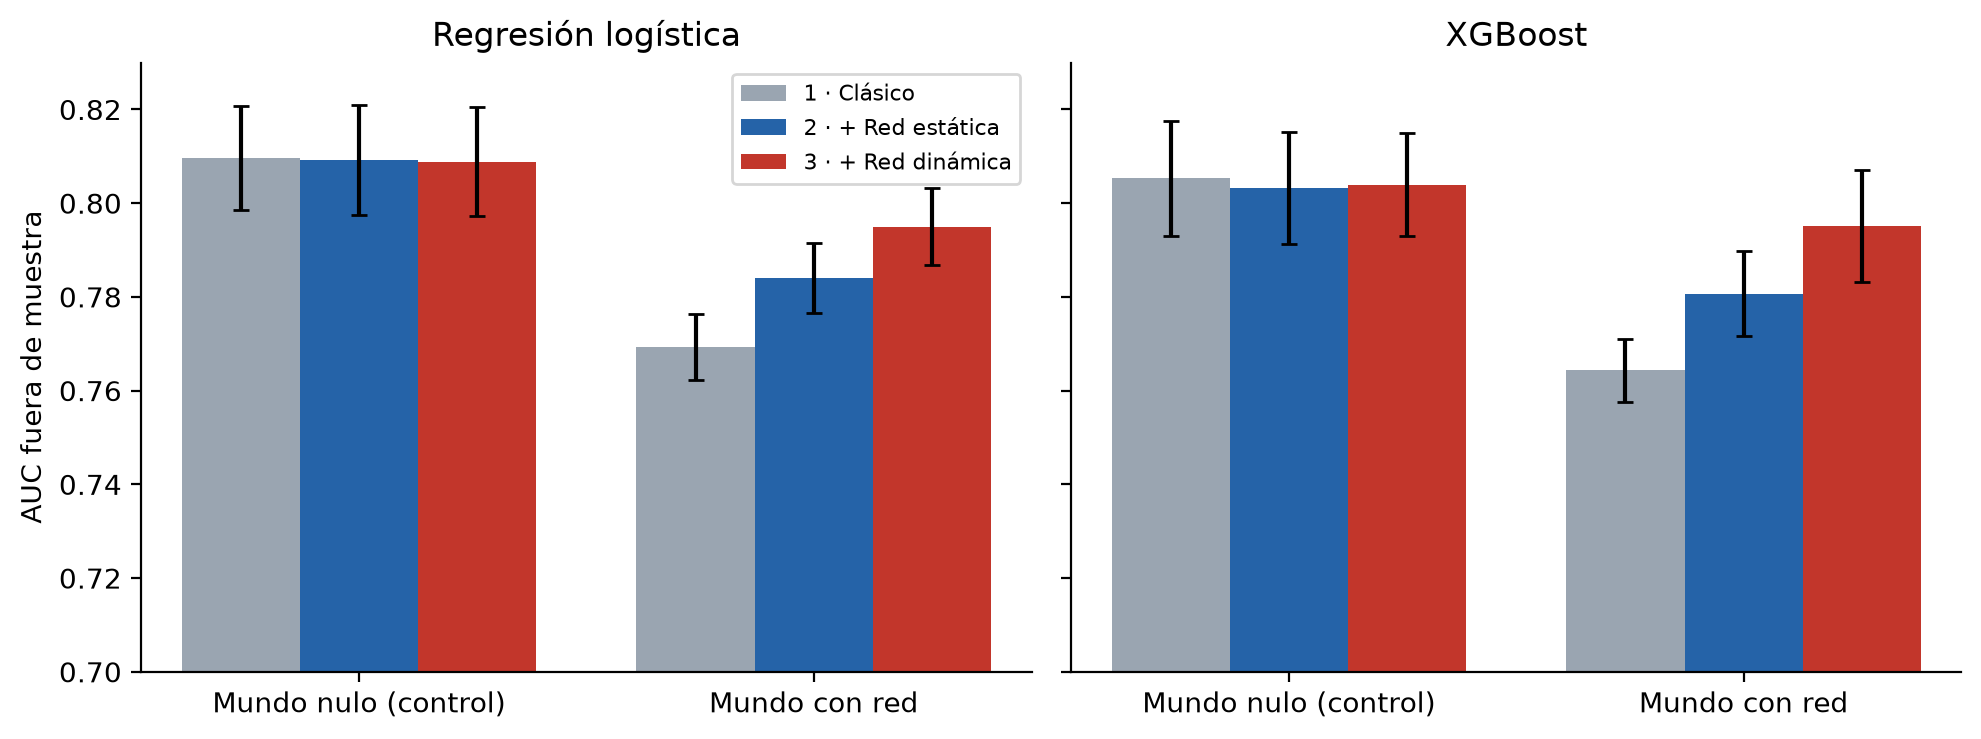
\includegraphics[width=0.78\textwidth]{tarea6_auc_niveles.png}
\begin{alertblock}{}
Régimen con red: las variables dinámicas mejoran sobre la red estática en
$\Delta\mathrm{AUC}=+0.011$ (logística) y $+0.014$ (XGBoost), con IC del 95~\% positivo
en 5 de 5 particiones. Régimen nulo: $\Delta\mathrm{AUC}\approx0$.
\end{alertblock}
\end{frame}

\begin{frame}{Mejoras pareadas por partición}
\centering
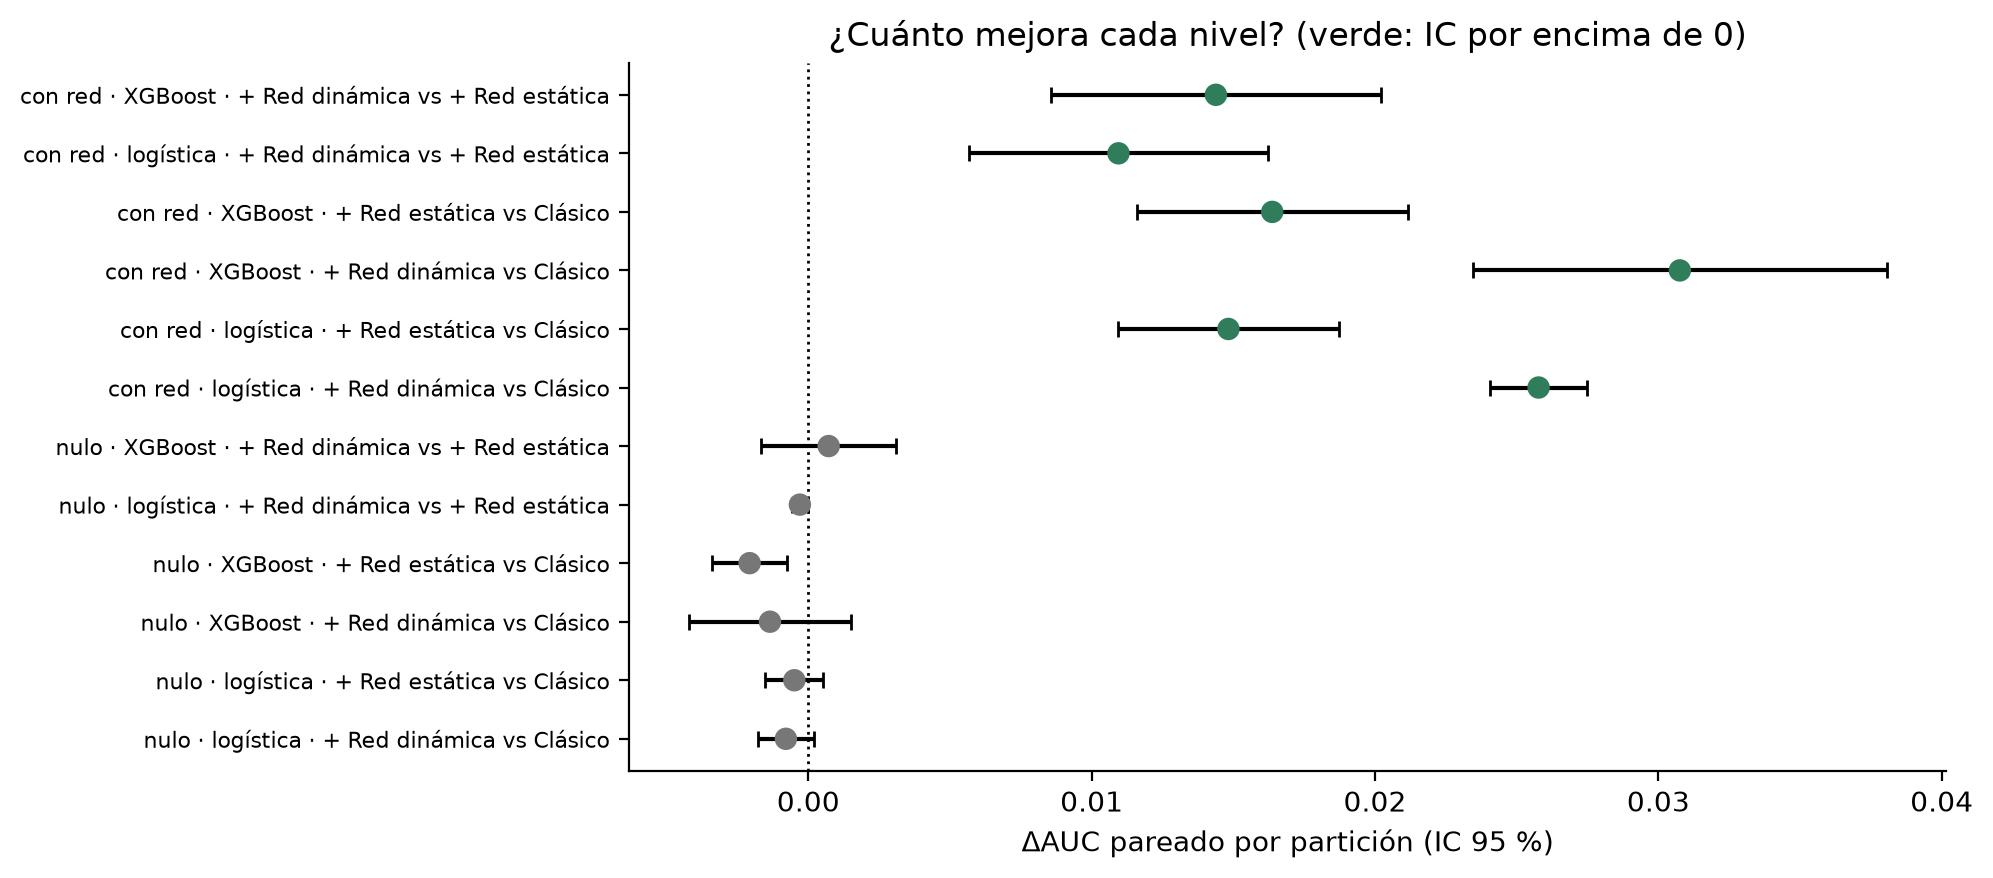
\includegraphics[height=0.78\textheight]{tarea6_mejoras.png}
\end{frame}

\begin{frame}{Sincronización, impago y quiebra de un empleador}
\begin{columns}[c]
\column{0.49\textwidth}
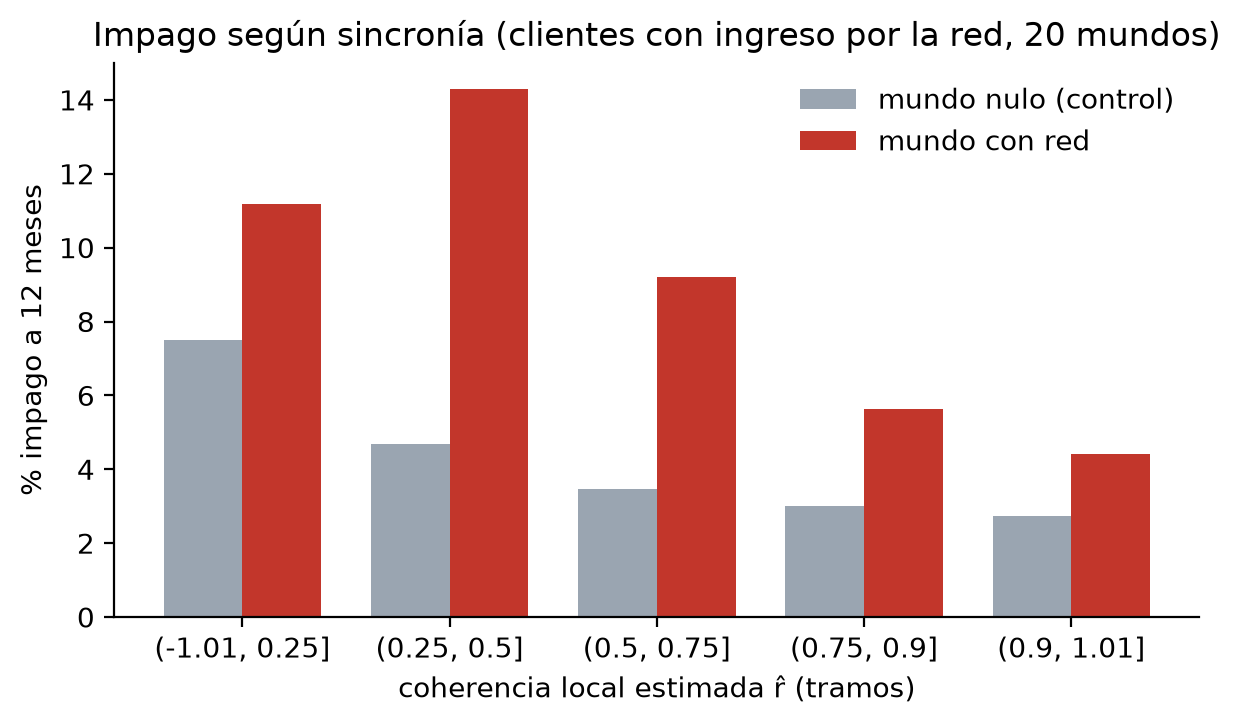
\includegraphics[width=\textwidth]{tarea6_impago_por_r.png}
\small Régimen con red: la tasa de impago pasa de 4.4~\% (clientes sincronizados) a
11–14~\% (desincronizados).
\column{0.49\textwidth}
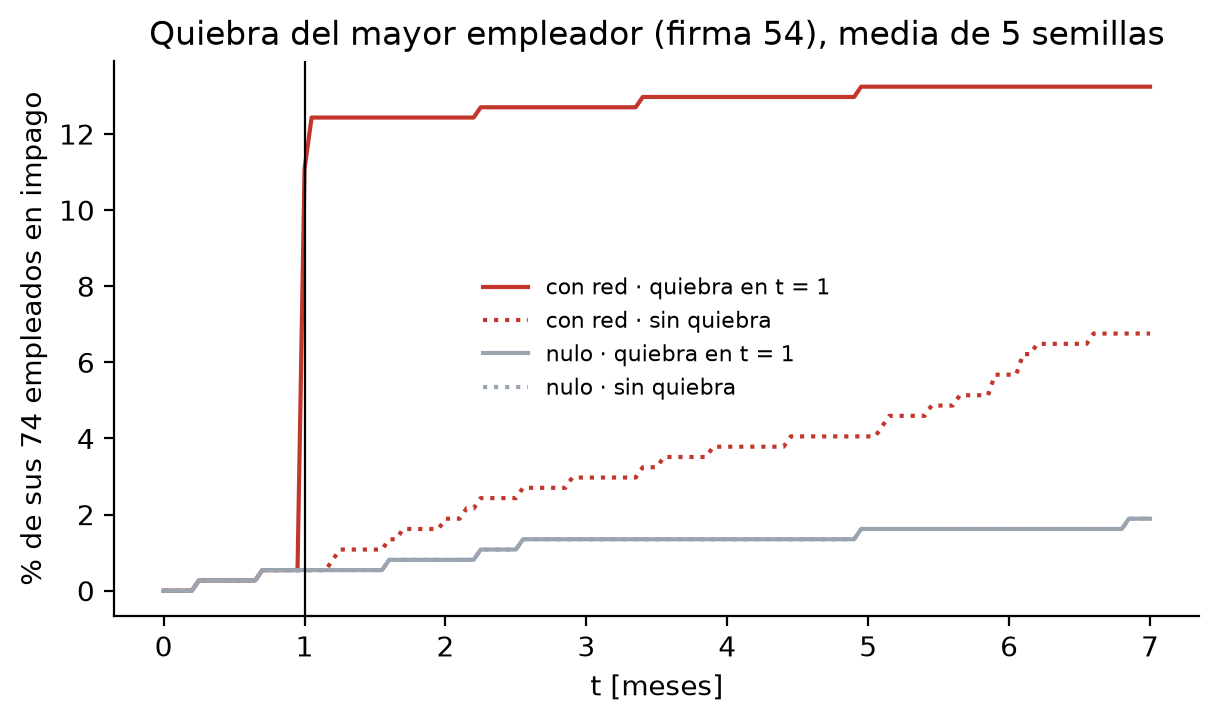
\includegraphics[width=\textwidth]{tarea6_quiebra.png}
\small Quiebra del principal empleador: el 12~\% de sus empleados incurre en impago de
inmediato; en el régimen nulo no se observa efecto.
\end{columns}
\end{frame}

\begin{frame}{Alcance e interpretación}
\small
\begin{columns}[T]
\column{0.48\textwidth}
\begin{block}{Conclusiones}
\begin{itemize}
\item Si el mecanismo existe, es \textbf{detectable} con los registros de
transacciones de que ya dispone un banco.
\item Las variables dinámicas aportan información no contenida en la red estática.
\item El control nulo descarta fugas de información.
\end{itemize}
\end{block}
\column{0.48\textwidth}
\begin{alertblock}{Limitaciones}
\begin{itemize}
\item No demuestra la existencia del mecanismo en una cartera real.
\item La magnitud del efecto depende de parámetros ilustrativos.
\item Se requiere una revisión bibliográfica sistemática.
\end{itemize}
\end{alertblock}
\end{columns}
\vspace{0.3cm}
\centering\textbf{Trabajo futuro}: aplicación del mismo procedimiento a datos reales
anonimizados.
\end{frame}

% ===================================================================
\section{Implementación}

\begin{frame}{Arquitectura del software}
\centering
\begin{tikzpicture}
\node[c=azul] (a) {\textbf{Interfaz} · \texttt{app/} (Streamlit, 9 páginas): presentación de resultados};
\node[c=verde,below=0.35cm of a] (b) {\textbf{Servicio} · \texttt{service.py}, \texttt{credit/service.py}: tablas para la interfaz};
\node[c=rojo,below=0.35cm of b] (c) {\textbf{Núcleo} · \texttt{model, integrate, spectral, cascades, ml/, world/, credit/}};
\node[c=orange,below=0.35cm of c] (d) {\textbf{Configuración y datos} · \texttt{configs/*.yaml}, \texttt{data/}, \texttt{models/}};
\draw[f] (a)--(b); \draw[f] (b)--(c); \draw[f] (c)--(d);
\end{tikzpicture}

\vspace{0.3cm}
\small Python 3.12 · NumPy/SciPy · pandas · scikit-learn · XGBoost · PyTorch Geometric ·
SHAP · Plotly · uv · pytest · ruff · Docker · GitHub Actions
\end{frame}

\begin{frame}{Aplicación web}
\begin{columns}[c]
\column{0.49\textwidth}
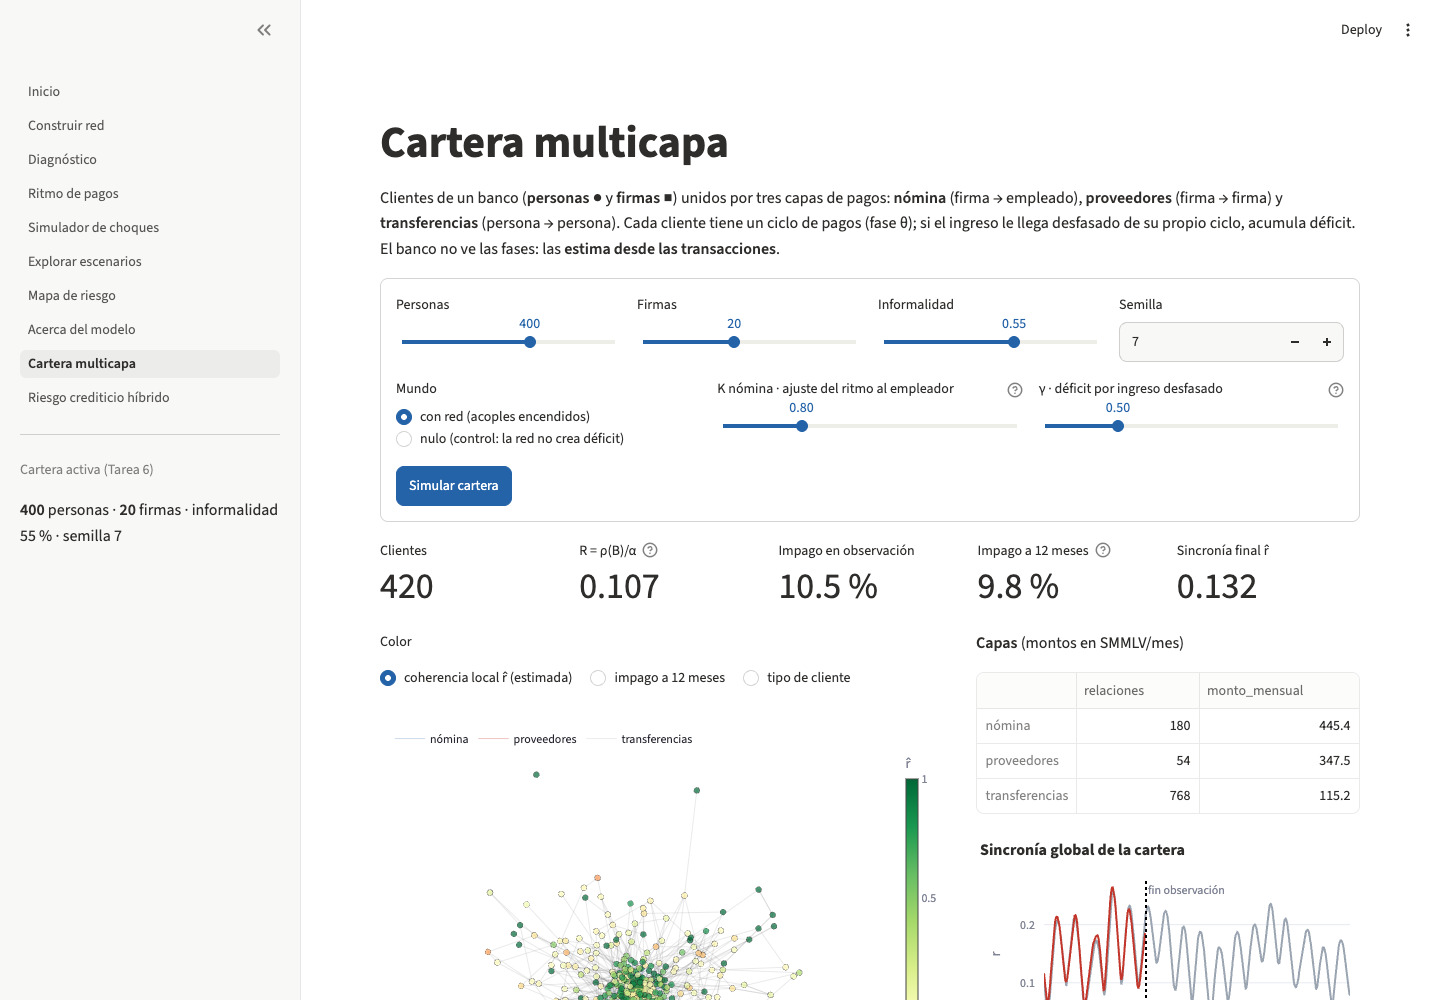
\includegraphics[width=\textwidth]{app_cartera.png}
\column{0.49\textwidth}
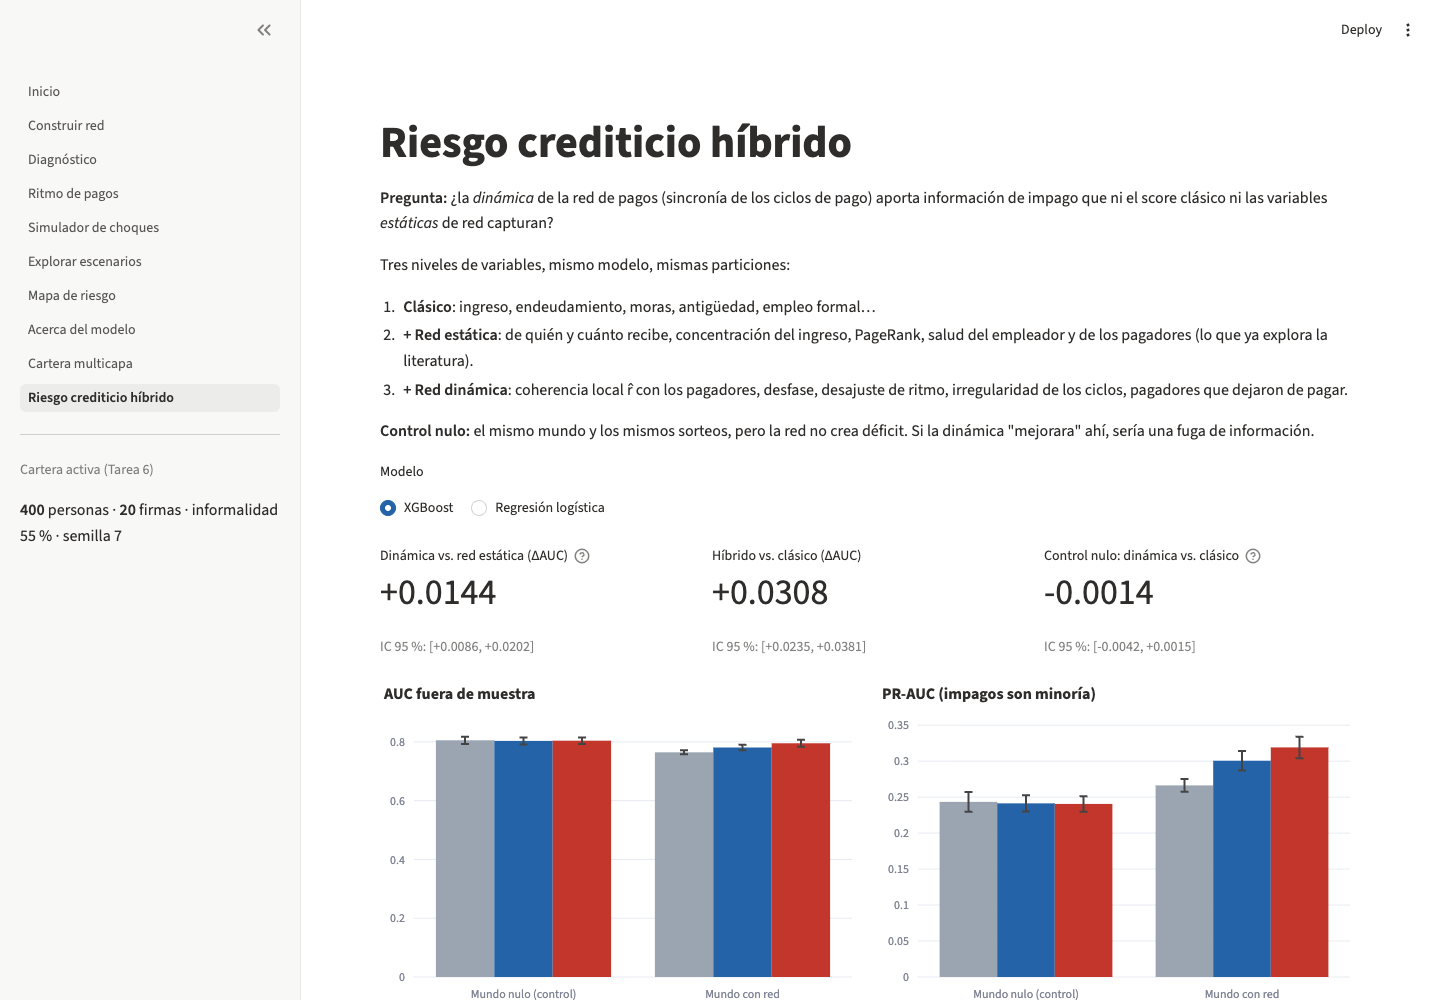
\includegraphics[width=\textwidth]{app_hibrido.png}
\end{columns}
\small Construir red · Diagnóstico · Ritmo de pagos · Simulador de choques · Explorar
escenarios · Mapa de riesgo · Acerca del modelo · \textbf{Cartera multicapa} ·
\textbf{Riesgo crediticio híbrido}
\end{frame}

\begin{frame}[fragile]{Ejecución}
\begin{verbatim}
uv sync                                    # instalación
uv run pytest                              # 127 pruebas
uv run streamlit run app/Inicio.py         # aplicación en localhost:8501

uv run pulso sweep  configs/sweep.yaml     # conjunto de datos, tarea 5
uv run pulso train  configs/train.yaml     # modelos, tarea 5
uv run pulso credit configs/credit.yaml    # experimento, tarea 6 (~20 s)

docker build -t pulso . && docker run -p 8501:8501 pulso
\end{verbatim}
\small Todos los parámetros residen en \texttt{configs/*.yaml}; la semilla explícita
garantiza la reproducibilidad.
\end{frame}

\begin{frame}[standout]
Gracias

\vspace{0.4cm}
\normalsize Documento completo: \texttt{docs/pulso\_guia\_completa.pdf}
\end{frame}

\end{document}
